% Este arquivo .tex será incluído no arquivo .tex principal. Não é preciso
% declarar nenhum cabeçalho

\section{Mensagem do Diretor da FEEC}

Caros Calouros de Engenharia de Computação,

É com grande satisfação que os recebemos na Unicamp e, em especial, na FEEC.

Nossa Faculdade traz em sua denominação duas Engenharias de imensa importância:
Engenharia de Computação e Engenharia Elétrica.  O mundo moderno está assentado
sobre alguns pilares, dois destes são a Informação e a Energia.  São exatamente
esses temas que orientam a FEEC em suas atividades de ensino, pesquisa e
extensão há 45 anos. Ter os melhores cursos do Brasil é uma grande
responsabilidade. Temos clareza de que isso foi construído por, principalmente,
contarmos com os melhores estudantes, ao que se associam excelentes professores
e uma infraestrutura que procura se manter renovada e atualizada.

Como vocês experimentarão, Engenharia de Computação é um curso exigente, que
requer empenho e espera desempenho dos estudantes. Em contrapartida, vocês terão
a oportunidade de participar da grande aventura do conhecimento, com
descobertas, talvez invenções, certamente com método.

O curso de Engenharia de Computação é compartilhado pela FEEC e pelo IC
(Instituto de Computação). Isso lhes abrirá, adicionalmente, a oportunidade de
conviver com professores e estudantes de outra unidade da Unicamp, o que é mais
uma oportunidade de conhecimento.

Mas a Universidade é muito mais do que o curso no qual vocês estão ingressando.
É um mundo em si, com todas as áreas do conhecimento, convivendo com pessoas dos
mais diferentes lugares, com arte e cultura, com debates e comemorações.
Aproveitem tudo isso, ao máximo, sem esquecer que vocês estão em uma escola
pública e gratuita, que sua permanência aqui se deve ao trabalho de milhões de
cidadãos do Brasil e, em particular, de São Paulo. Honrem o trabalho de todas
essas pessoas, dando o melhor de si, com ética e dedicação, seja durante o
curso, seja daqui a pouco, quando já forem profissionais.

\begin{wrapfigure}{l}{0.4\textwidth}
    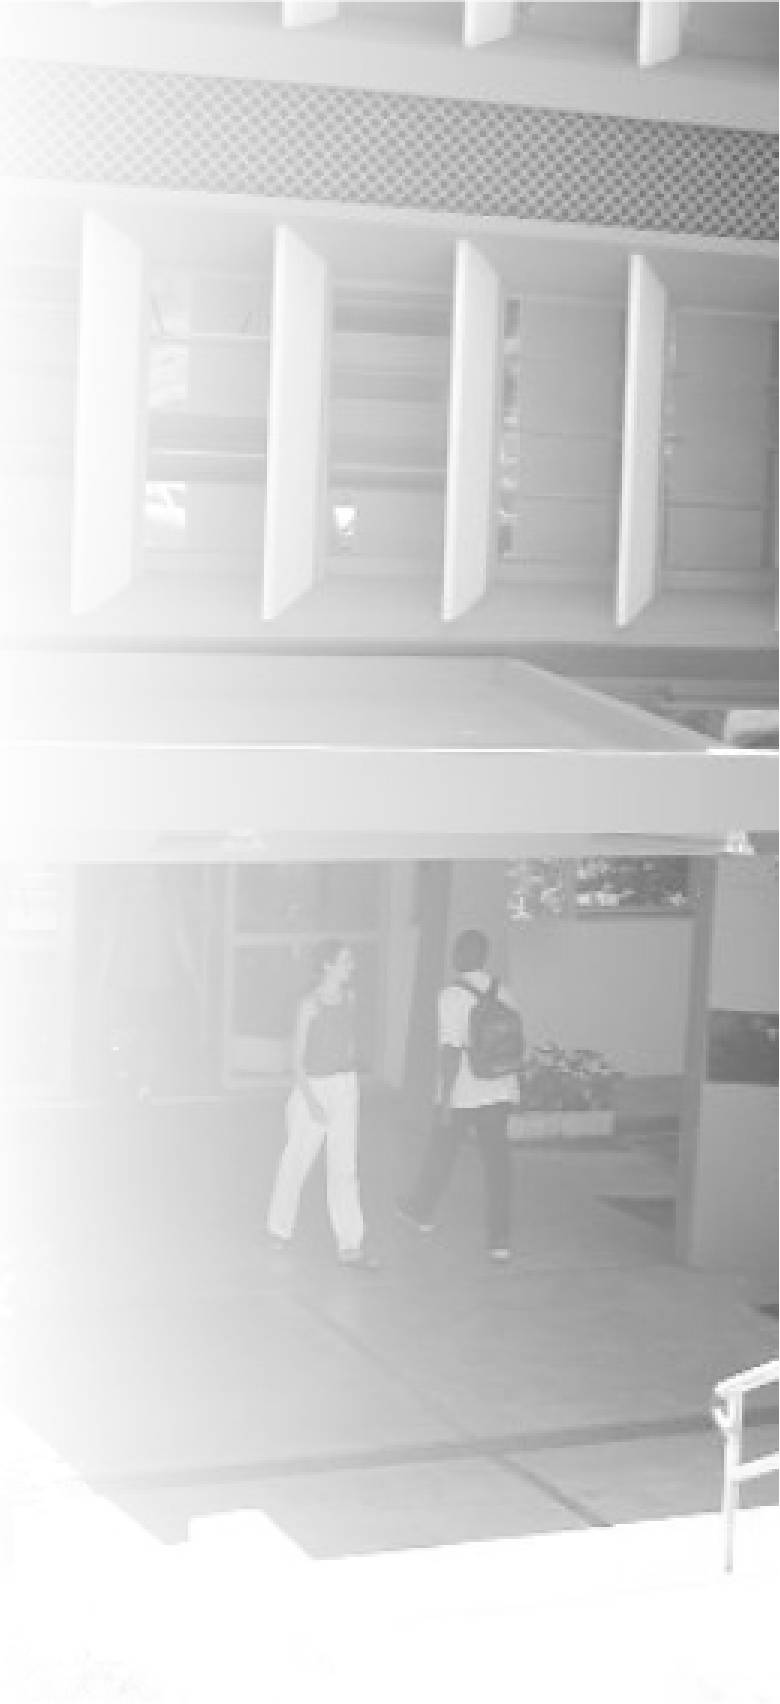
\includegraphics[scale=0.30, keepaspectratio=true]{img/imgs/3-feec/feec.jpg}
\end{wrapfigure}

Bem-vindos à FEEC e a diretoria e as coordenações de curso estarão sempre à
disposição para ajudar no que for possível.

José Antenor Pomilio

Diretor da FEEC
